%-------------------------------------------------------------------------------
\section{Introduction}
%-------------------------------------------------------------------------------
Web application developers today have more incentives than ever to provide better privacy for their
users.
%
Laws such as the EU's General Data Protection Regulation (GDPR)~\cite{eu:gdpr} and California's
Consumer Privacy Act (CCPA)~\cite{ca:privacy-act} codify users' right to be forgotten, and demand
applications to support privacy-granting user unsubscription.
%
Growing legal consequences for data breaches push applications to minimize the amount of
compromising data they retain~\cite{breach:amazon,breach:twitter, breach:fb, breach:marriott,
breach:quora}.

Although developers should support better privacy policies, doing so is challenging.  They must
perform data privacy transformations to adhere to the privacy policy, while ensuring that the
application retains data required for legal purposes or to preserve application utility, and without
violating application invariants.
%
For example, unsubscription of one user should not allow another user to view content that she
originally could not access.

Transformations that achieve better user privacy requires careful handling of data deletion,
anonymization, and structural decorrelation, where developers must consider how to handle both
clearly identifying content (\eg usernames), and also structural correlations between data records
that can identify the user.
While these transformations do not enable formal privacy \emph{guarantees}, developers can improve the state of privacy in applications today by reasoning about often subtle identifying correlations.

For example, unsubscriber users' public running routes correlated with the same location can
reidentify the users' hometowns or homes, and the users themselves, even if the route's creator is
anonymized. Anonymized posts on Reddit correlated with the same subreddit, particularly if the
subreddit has very few subscribers, can be associated back to a single user; and
content correlated with the same group of people (\eg papers that have the same paper conflicts in
HotCRP, or posts liked by the same set of friends) can identify a user via their community.

As privacy policies become more complex, the burden of implementing the corresponding privacy
transformation correctly grows as well.
Consequently, today's applications often support only coarse-grained and simple privacy policies,
implemented using ad-hoc methods.

We next describe a wide range of privacy transformations, some from existing applications' privacy policies,
and others that demonstrate the potential for better, more nuanced privacy policies. Implementing
these transformations using ad-hoc methods places undue labor on the developer and, as policies grow
more complex, becomes more error-prone.

To systematically address these challenges, we propose \emph{data masking}, a new framework for
specifying and implementing privacy transformations for privacy policies.
%
With data masking, developers specify privacy transformations required in privacy policies, \eg
unsubscription, as \emph{data masks}. A data mask constrains the state of the entity relationship
graph embedded in database-backed applications (\eg encoded by foreign key relationships).
%
Data masking tools take a data mask and a top-level entity to mask (\eg the user to
unsubscribe), and automatically translates the mask into the appropriate database transformations to
achieve the masked entity graph state. With these tools, developers reason only about constraints on
the entity graph, and avoid the labor of manual mask implemention.

\subsection{Privacy Transformations Today and Beyond}
A survey of current applications' privacy policies reveal a set of common privacy transformations performed during user unsubscription
%~\cite{facebook:privacy, twitter:privacy, hotcrp:privacy, reddit:privacy,
%github:privacy, hackernews:privacy, strava:privacy, linkedin:privacy, stackoverflow:privacy,
%wikipedia:privacy, amazon:privacy, prestashop:privacy, spotify:privacy, lobsters:privacy}:
\begin{itemize}[nosep]
    \item Keep user's public contributions publicly and indefinitely available (\eg Wikipedia,
        StackOverflow, Strava)~\cite{wikipedia:privacy, stackoverflow:privacy, strava:privacy}.
    \item Keep user's contributions directly shared with another unanonymized and visible to the recipient user (\eg Facebook,
        LinkedIn, Twitter)~\cite{twitter:privacy, facebook:privacy, linkedin:privacy}.
    \item Keep user contributions visible to the intended audience, but anonymized by reassociation with a global
        placeholder user (\eg GitHub, Reddit, Lobsters)~\cite{github:privacy, reddit:privacy,
        lobsters:privacy}.
    \item Keep certain user contributions unanonymized and visible to its intended audience (\eg
        HotCRP, Lobsters, Wikipedia, HackerNews)~\cite{hotcrp:privacy, lobsters:privacy,
        hackernews:privacy, wikipedia:privacy}.
    \item Delete user contributions on user profile or feed (\eg Facebook,
        Twitter)~\cite{facebook:privacy, twitter:privacy}.
    \item Retain personal information for legal or necessary business purposes (all web applications).
\end{itemize}

We can also imagine applications supporting more flexible and nuanced policies, such as
\begin{itemize}[nosep]
    \item Keep user's contributions, but associate each contribution with a different user account
        (\eg reassociate each of a user's HotCRP reviews with a separate account).
    \item Remove users' contributions that have the same public characteristic (\eg remove the user's
       posts on Reddit if they share a common tag).
    \item Remove users' contributions that have the same public characteristic, but only if this
        characteristic was created by the user (\eg remove the user's posts on Reddit if they share
        a user-customized tag).
    \item Remove users' contributions if they comprise more than $p$
            percent of the contributions with the same public characteristic (\eg remove the user's
            posts on Reddit with tag $t$ if these posts comprise more than 10\% of all posts with
            tag $t$).
    \item Encrypt the user's profile and reassociate their contributions with an anonymous
        profile after the user account has been inactive for a fixed period of time;
        restore the user's profile and reassociate their contributions if the user ever logs back in.
\end{itemize}
These envisioned policies allow applications to, \eg be more selective in the data and structural
correlations that it retains or removes upon unsubscription, and add new policies that provide
better privacy for users' data even if the user does not manually unsubscribe, which many applications
fail to do today.

\subsection{Data Masking: A New Approach to Privacy Policies}
\begin{figure}[t!]
    \centering
    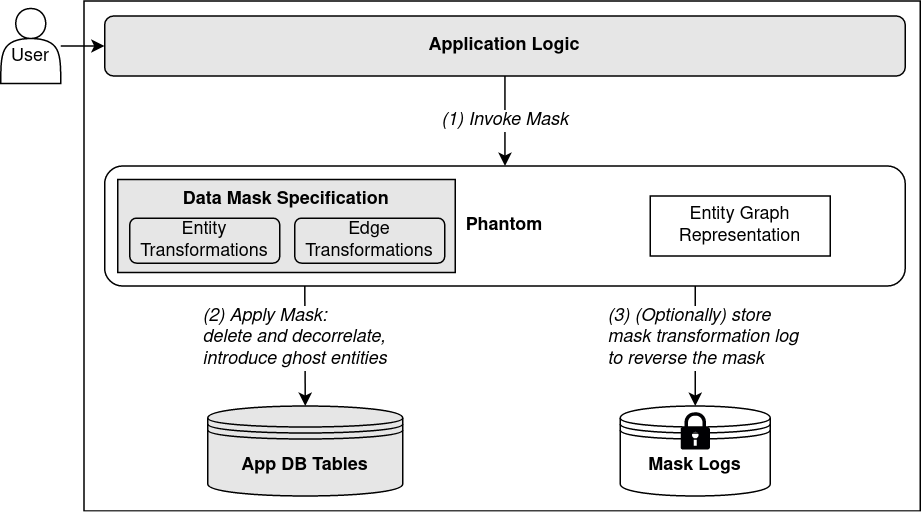
\includegraphics[width=0.5\textwidth]{img/impl}

    \caption{Data masker architecture. Developers specify grayed-out components.}
    \label{fig:arch}
\end{figure}

To enable developers to better support existing and new privacy policies without onerous manual
labor, we propose \emph{data masking}.
%
Data masking is a new systematic approach that helps developers generate
\emph{data masks}---concrete privacy transformations---for database-backed web applications. The
developer provides a high-level, declarative specification of the desired privacy policy, and a data
masking implementation masks the database according to the policy.

Data masking relies on the key observation that applications already encode entity relations in an
\emph{entity graph} encoded via \eg foreign key relationships, and privacy transformations impose
restrictions on the content and structure of this graph. Unsubscription, for example, transforms
this graph to comply with particular constraints of the privacy transformation for account deletion.

With data masking, the developer specifies desired privacy transformations as a \emph{data mask}.
Using their application expertise, the developer selects from a menu of possible transformations
(Section~\ref{sec:policies}) that can be performed on entity graph edges and entity nodes (\eg
foreign key relationships and table rows). The chosen set of transformations---the data
mask---determines the structure of the entity graph after the mask is applied to the targeted entity
(\eg the user to unsubscribe).

The menu of entity graph transformations rely on the concept of \emph{ghost entities}, namely
transformed and potentially duplicated versions of real entities. Decorrelating and modifying
entities in the entity graph can expressed via transformations that restructure the entity graph
with edges to ghost entities that have replaced real ones.

Importantly, data masks perform \emph{reversible} transformations, allowing developers to support
privacy-granting transformations beyond permanent and irrevokable unsubscription (\eg
user data expiration or timeouts).

Data masking tools take a data mask and the top-level entity to mask, and automatically generate and
apply the mask via the appropriate database transformations that would be laborious to implement
manually.
%(\eg decorrelate post entities from user entities by rewriting the foreign key relationship to a
%newly generated ghost user entity).
As an initial design and prototype for such a tool, we create \sys, which sits between application
logic and its database (Figure~\ref{fig:arch}). We show that \sys achieves reasonable performance,
and can automatically and systematically apply data masks to application data given a high-level
mask specification.
%To help developers of new and existing applications support privatization transformations, we
%propose \sys, which makes the key insight to model application data as an abstract \emph{entity
%graph}, and represent privatization transformations as transformations of this graph that render
%particular entities private.

\iffalse
Web applications today own, process, and store user data~\cite{nytimes:fb, npr:data}. This places a
great responsibility on application developers to transparently convey to users how they manage this
data via their privacy policies and terms of use.
%
\ms{next sentence doesn't follow: privacy policies + ToS doesn't imply data masks.}
Recent developments have renewed efforts to improve the state of data management in web
applications, creating incentives to support different forms of \emph{data masks}.

For example, applications mask data to hide a users' identity, performing privacy-preserving user
unsubscription from a service as mandated by laws such as the EU's General Data Protection
Regulation (GDPR)~\cite{eu:gdpr} and California's Consumer Privacy Act (CCPA)~\cite{ca:privacy-act}
that codify users' rights to data ownership and right to be forgotten. Unsubscription motivates a
need for an identify-revealing resubscription transformation, making it easy for users to return
instead of forcing users to permanently give up their accounts.

Growing incentives to keep as little compromising data as possible in case of a data
breach~\cite{breach:amazon,breach:twitter, breach:fb, breach:marriott, breach:quora} prompt
applications to mask stale or inactive users' data via anonymization or deletion. Similarly,
applications want to mask data that is stored in backups, or given to others for data processing.

%Data masks also go beyond just masking user data: applications apply masks to moderate
%harmful data (\eg inappropriate content or misinformation) that hide or modify data
%contents~\cite{contentmod, sasb}, and face increasing pressure from users who want to
%hold them legally liable for appropriately moderating content~\cite{nytimes:230}.

Properly specifying and implementing these various data masks is challenging. Masks are necessarily
application-specific and require the developer to reason about and handle complex data correlations.
For example, developers must selectively retain unsubscribing users' data for legal or application
purposes, while de-identifying this data as much as possible and maintaining application semantics.
Today's applications often support only coarse-grained masks implemented with ad-hoc methods,
resulting in a lack of a clear specification of exactly what and how the mask transforms data.

To help developers of new and existing applications support clearly specified data masks, we propose
\sys, a framework that, given only a high-level, declarative specification of the relationships
between entities in a database, generates and applies complex transformations that would be
laborious to implement manually. We observe that applications already encode entity
relations in an \emph{entity graph} via foreign key relationships, and this graph provides a means
for \sys to systematically reason about and automate a variety of data masks.
%To help developers of new and existing applications support privatization transformations, we
%propose \sys, which makes the key insight to model application data as an abstract \emph{entity
%graph}, and represent privatization transformations as transformations of this graph that render
%particular entities private.

With \sys, developers specify a \emph{mask policy} by choosing from a menu of provided edge and node
transformations. To determine an appropriate policy, developers introduce \emph{ghost entities} in the entity graph, which allow the mask to both retain, decorrelate, modify,
and remove data. The policy acts as a specification for the masked state of any instance of the
entity graph. When invoked with a particular mask policy, \sys automatically and systematically
applies transformations to the current entity graph instance to achieve this specified state.

We evaluate an initial prototype for \sys, finding that \sys automatically applies
data masks efficiently, and that practical policies can be expressed with low burden for application
developers.
\fi

\iffalse
%\begin{figure*}[ht!]
%    \centering
%    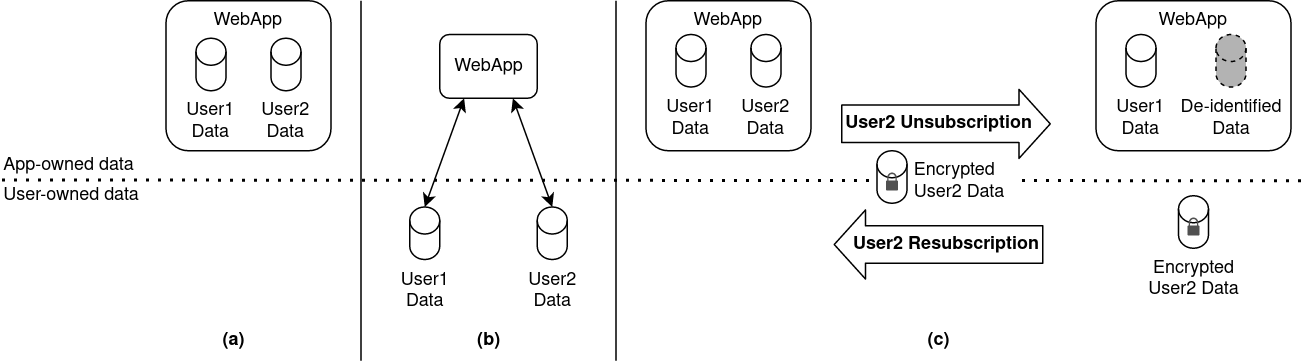
\includegraphics[width=\textwidth]{img/worlds}
%
%    \caption{\textbf{(a)} The current web application paradigm, in which applications maintain and
%    own user data; \textbf{(b)} A paradigm that decouples user data from web applications, giving users ownership of their data;
%    \textbf{(c)} \name, which allows users to switch between privacy-preserving unsubscribed mode (right) and identity-revealing subscribed mode (left).}
%    \label{fig:world}
%\end{figure*}
%
Web applications today own, store, and sell user data, often without the user's knowledge or
explicit consent~\cite{nytimes:fb, npr:data}. This both violates users' right for privacy, and has
dangerous consequences for both users and application developers as data leaks lead to loss of
livelihoods and lawsuits~\cite{breach:amazon,breach:twitter, breach:fb, breach:marriott,
breach:quora}.
%Granting web applications complete ownership of personal data clearly fails to
%protect users' privacy.

Although users want stronger privacy, completely decoupling user data from applications results in a
potentially even less desirable world. While possible~\cite{solid, amber, w5, blockstack, bstore}, such a
model hinders service-side computation and application performance, and requires users to manage
long-time security and storage of their data, leading to a lack of adoption in practice (Section~\ref{sec:related}).

This paper proposes \name, a new paradigm that grants users flexible privacy when using web
applications, balancing users' desire for privacy with their desire for application utility. In
\name, users subscribe to applications by granting a time-limited lease to their data, with the
provision that the application may retain only de-identified information once the user unsubscribes.
Users flexibly switch between a privacy-preserving unsubscribed mode and an identity-revealing
subscribed mode at any time without permanently losing their data. \name contrasts
with the current web application paradigm for data ownership, in which applications have complete
ownership, and the other extreme in which the user has complete data ownership.% (see Figure~\ref{fig:world}).

\name benefits users: they can choose privacy at any time, without
permanently losing their accounts or affecting the utility of the applications for others.  Just as
importantly, \name also benefits application developers. Recent laws such as the
European Union's General Data Protection Regulation (GDPR)~\cite{eu:gdpr} and California's Consumer
Privacy Act (CCPA)~\cite{ca:privacy-act} codify users' rights to data ownership, granting users the
right to request erasure of information related to them. Supporting \name enables
applications to comply with these legal mandates, while still allowing its departing users to easily
come back: if applications must let users leave, it is in their best interest to make it easy for
them to return.

Furthermore, applications can continue to operate using their current revenue model, maintaining
performance, reliability, and utility for their users.  Because applications retain use of
subscribed users' data, and de-identified data of unsubscribed users, applications optimize the
amount of data available to generate profit and provide utility for subscribed users. The
application holds only identifying data for subscribed users, reducing the amount of
compromising data in the system to only those users who have actively agreed to temporarily give up
their privacy.

Realizing \name poses a number of technical challenges.
Unsubscription and resubscription requires complex and fragile data transformations: developers must
selectively retain unsubscribed users' data for legal or application purposes while properly
de-identifying this data, a non-trivial task in the face of subtle inference attacks (\eg tags on a
user's post can identify the user). De-identification and data removal needs to be reversible,
allowing the user to resubscribe at any time to their last-known subscribed state.

To make \name a reality, we model application data as an abstract \emph{entity graph}, and
represent unsubscription and resubscription as transformations of this graph.
\emph{Ghost entities} allow transformations to achieve both data retention and de-identification,
and declarative \emph{ghost policies} specify reversible transformations upon unsubscription.
We design and implement \sys, a practical system that systematically automates this transformation for new and existing applications, helping developers realize the \name paradigm without onerous labor.
%that takes a developer-specified unsubscription policy for the application's entity
%graph, and ensures that
%that requires developers only to specify an abstract unsubscription policy on the
%helps developers of databased-backed web applications automatically achieve correct, privacy-compliant user unsubscription and
%resubscription without onerous labor.
\fi
